\documentclass[14pt,a4paper,openright,twoside]{extreport}
\usepackage[utf8]{inputenc}
\usepackage[english]{babel}
\usepackage[inner=2cm,outer=2cm,top=2cm,bottom=2cm]{geometry}
\usepackage{graphicx}
\usepackage{amsmath}
\usepackage{amsfonts}
\usepackage{pifont}
\usepackage{textcomp}
\usepackage{amssymb}
\usepackage{epstopdf}
\usepackage[onehalfspacing]{setspace}
\usepackage{tabularx}
\usepackage{mathrsfs}
\usepackage{rotating}
\usepackage{caption}
\usepackage[usenames,dvipsnames]{xcolor}
\usepackage{fancyref}
\usepackage{subcaption}
\usepackage{braket}
\usepackage{color}
\usepackage{float}
\usepackage{enumerate}
\usepackage[pagebackref]{hyperref}
\usepackage{afterpage}
\usepackage[makeroom]{cancel}
\usepackage{mathtools}

\usepackage{fancyhdr}
\pagestyle{fancy}

\fancyhead{}
\fancyhead[RE, LO]{{\nouppercase{\rightmark{From: Minh Nguyen \ding{120} Pranjal Dhole}}}}
\fancyhead[LE, RO]{\thepage}
\renewcommand{\headrulewidth}{0.4pt}

\fancyfoot{}
\fancyfoot[RE, LO]{{\nouppercase{\leftmark{MAS-SS2017 | Hochschule Bonn-Rhein-Sieg}}}}
\fancyfoot[LE, RO]{Date: 04.05.2017}
\renewcommand{\footrulewidth}{0.4pt}
\graphicspath{{images/}}
\newcommand\fnurl[2]{%
    \href{#2}{#1}\footnote{\url{#2}}%
}
\hypersetup{
    pdftoolbar=true,        % show Acrobat’s toolbar?
    pdfmenubar=true,        % show Acrobat’s menu?
    pdffitwindow=false,     % window fit to page when opened
    pdfstartview={FitH},    % fits the width of the page to the window
    pdftitle={Evolutionary Computation: Theory and Application Homework},    % title
    pdfauthor={Pranjal Dhole},     % author
    pdfsubject={Review},   % subject of the document
    pdfcreator={Pranjal Dhole},   % creator of the document
    pdfproducer={Pranjal Dhole}, % producer of the document
    pdfkeywords={Evolutionary Computational Theory and Application}, % list of keywords
    pdfnewwindow=true,      % links in new window
    colorlinks=true,       % false: boxed links; true: colored links
    linkcolor=MidnightBlue, % color of internal links (change box color with linkbordercolor)
    citecolor=Thistle,        % color of links to bibliography
    filecolor=magenta,      % color of file links
    urlcolor=Sepia           % color of external links
}
%%%%%%%%%%%%%%%%%%%%%%%%%%%%%%%%%%%%%%%%%%%%%%%%%%%%%%%%%%%%%%%%%%%%%%%%%%%
%specific
\raggedbottom
%%%%%%%%%%%%%%%%%%%%%%%%%%%%%%%%%%%%%%%%%%%%%%%%%%%%%%%%%%%%%%%%%%%%%%%%%%%
\pagenumbering{arabic}
\begin{document}
%%%%%%%%%%%%%%%%%%%%%%%%%%%%%%%%%%%%%%%%%%%%%%%%%%%%%%%%%%%%%%%%%%%%%%%%%%%
\begin{center}
\LARGE{\underline{Evolutionary Computation: Theory and Application}}\\
\LARGE{\underline{Assignment - 02}}
\section*{\underline{Travelling Salesman Problem}}
\end{center}

\subsection*{\textbf{Parameter values used for computation and analysis:}}
number of cities: 100 \\
Population size in each generation: 200  \\
mutation rate: $ 0.01$ \\
crossover rate $ 0.9$ \\
elitism: Best fitness \\
number of generations: 1500 \\

%Threshold for crossover: 0.6
\subsection*{\textbf{Randomly initialized population}}
\begin{figure}[H]
    \begin{center}
        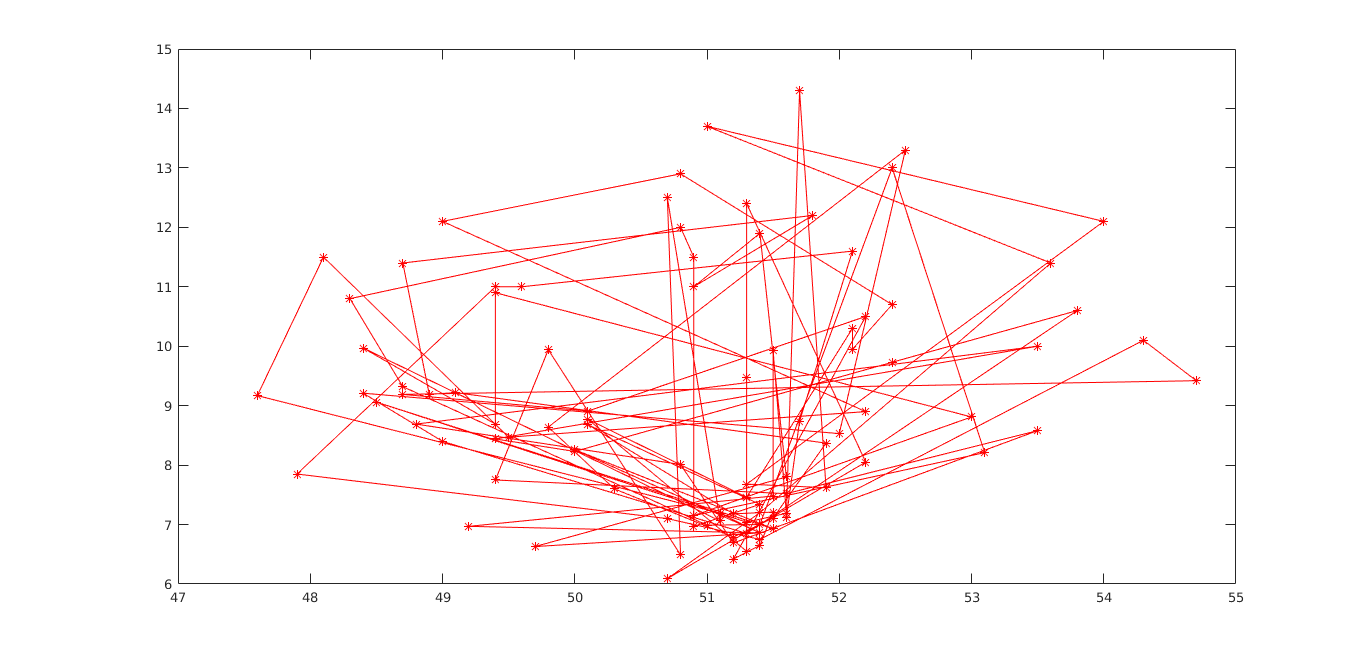
\includegraphics[width=\textwidth]{tspmap_randomcross_neighbormutate_1500_before.png}
        \caption{\small{Edge map of individual with the best fitness from the initialized population}}
        \label{mapinitalize1500}
    \end{center}
\end{figure}
\subsection*{\textbf{Best fitness after 1500 generations}}
\begin{figure}[H]
    \begin{center}
        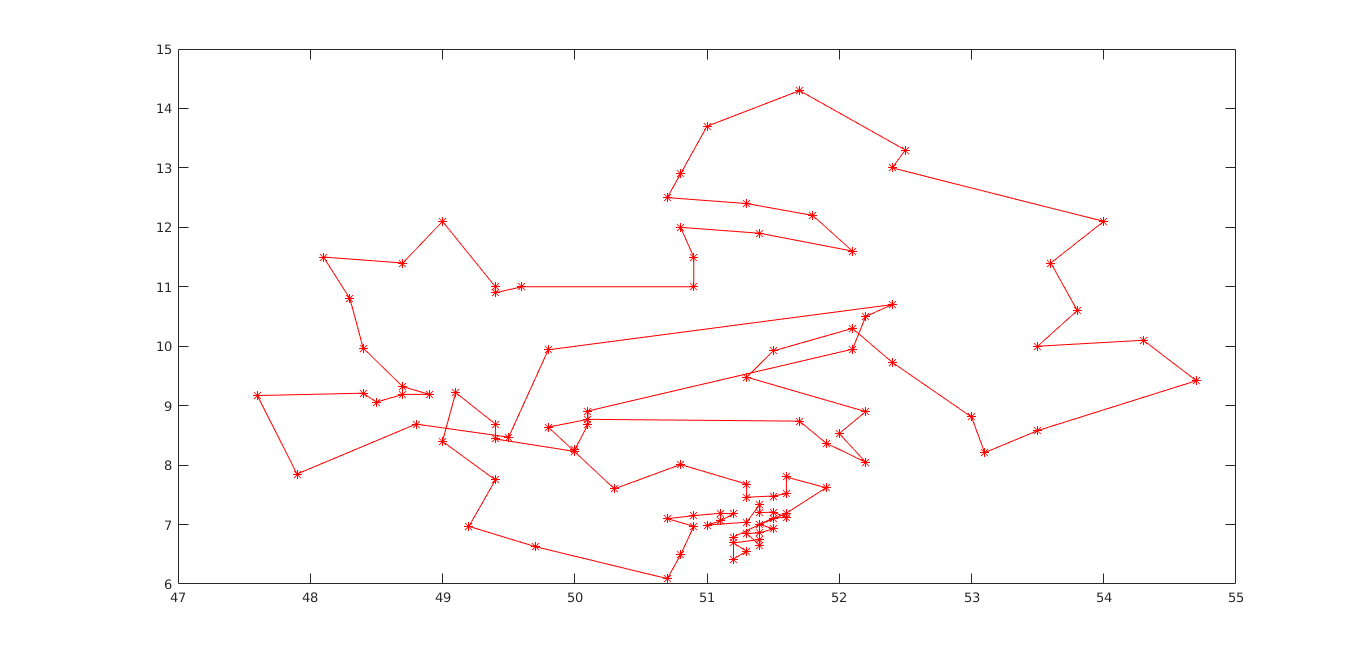
\includegraphics[width=\textwidth]{tspmap_randomcross_neighbormutate_1500_after.png}
        \caption{\small{Edge map of individual with the best fitness after 1500 generations, using random crossover and neighbor swapping mutation.}}
        \label{mapsolution1500}
    \end{center}
\end{figure}

\begin{figure}[H]
    \begin{center}
        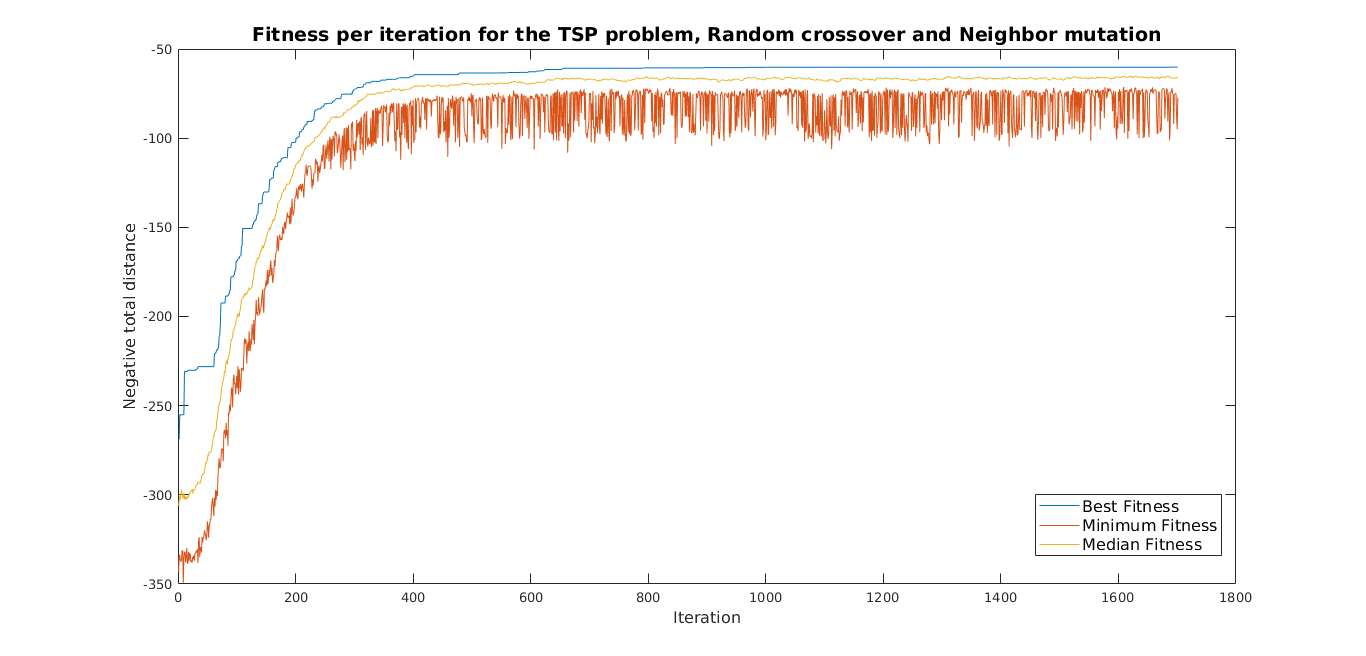
\includegraphics[width=\textwidth]{tspmap_randomcross_neighbormutate_1500_fitness.png}
        \caption{\small{Evolution of fitness in each generation. We see that all best, mean and minimum fitness increases gradually over generations before we converge to a solution. This means that we have a reasonably well-conditioned mutation rate for the problem. The algorithm looks for maxima on the fitness landscape, thus our distance values have negative sign.}}
        \label{fitness1500}
    \end{center}
\end{figure}

\newpage
\section*{Experimentation with mutation and crossover mechanisms}

number of cities: 100 \\
Population size in each generation: 200  \\
elitism is present \\
number of generations: 800 \\
crossover rate: 0.9 \\
mutation rate: 0.01


\subsection*{Experimentation Description}
\subsubsection*{Setup}
\begin{itemize}
    \item Two mutation and two crossover methods are implemented
    \item Each combination of mutation and method is run 30 times
    \item The best fitness of the population is recorded for each iteration, and the median over 30 runs is recorded.
    \item The child with the best fitness of 30 runs is also recorded for each combination of crossover and mutation method.
    \item The same initialization is used for each combination of techniques.
\end{itemize}

\subsubsection*{Mutation methods}
Each gene is chosen to mutate or not using the mutation rate as the probability.
\begin{itemize}
    \item Order change: if gene mutate, it will swap place with a randomly selected gene in the genome.
    \item Neighbor swapping: if gene mutate, it will swap place with the adjacent gene (wrap around).
\end{itemize}


\subsubsection*{Crossover methods}
\begin{itemize}
    \item Cycle crossover: implement the algorithm as described on the tutorial from \fnurl{rubicite.com}{http://www.rubicite.com/Tutorials/GeneticAlgorithms/CrossoverOperators/CycleCrossoverOperator.aspx}
    \item Random crossover: a set number of genes are chosen randomly from first parent, then the rest are picked from the second parent so that all genes has an unique value (all cities are traveled only once).
\end{itemize}


\subsection*{\textbf{Mapping of best solution for }}
\begin{figure}[H]
\begin{center}
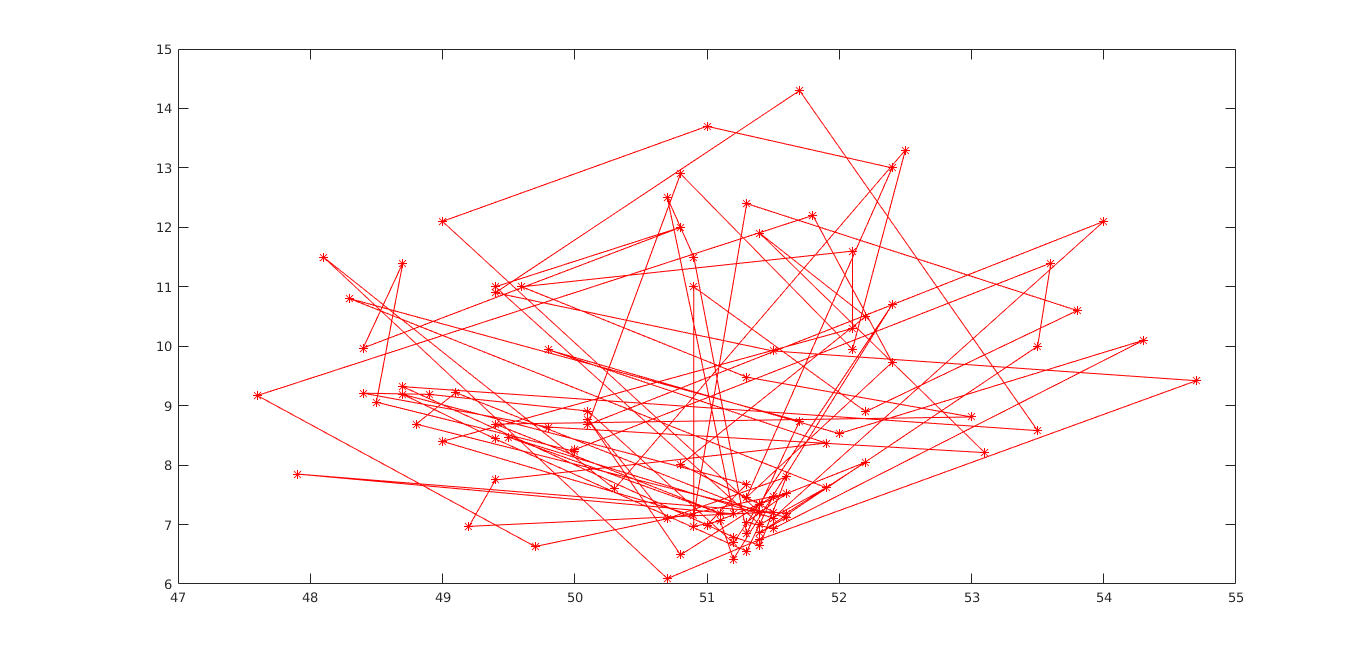
\includegraphics[width=\textwidth]{tspmap_randomcross_neighbormutate_800_before.png}
\caption{\small{Edge map of individual with the best fitness from the initialized population}}
\label{genesis}
\end{center}
\end{figure}
\subsection*{\textbf{Best fitness after 800 generations}}
\begin{figure}[H]
\begin{center}
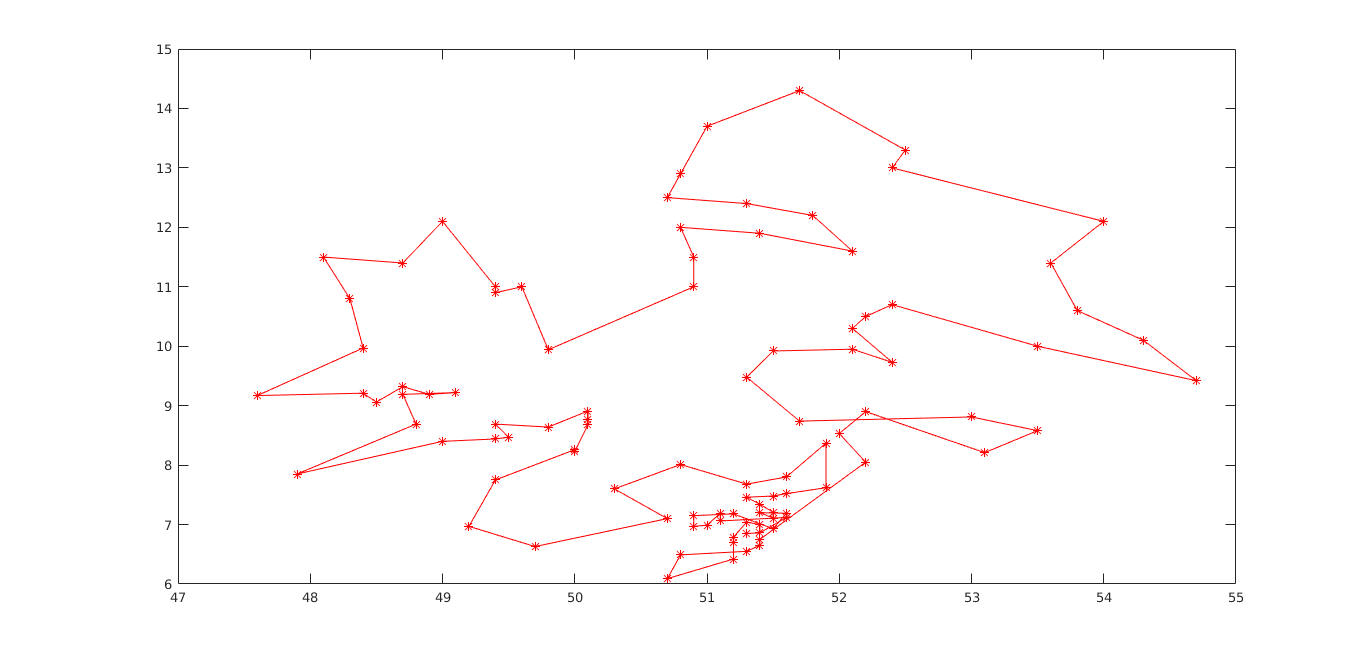
\includegraphics[width=\textwidth]{tspmap_randomcross_neighbormutate_800_after.png}
\caption{\small{Best solution from 30 runs of each combinations for 800 generations each. The solution was acquired using a combination of random crossover and neighbor swapping mutation. The total distance for this solution is $57.9948$.}}
\label{converge}
\end{center}
\end{figure}

\begin{figure}[H]
\begin{center}
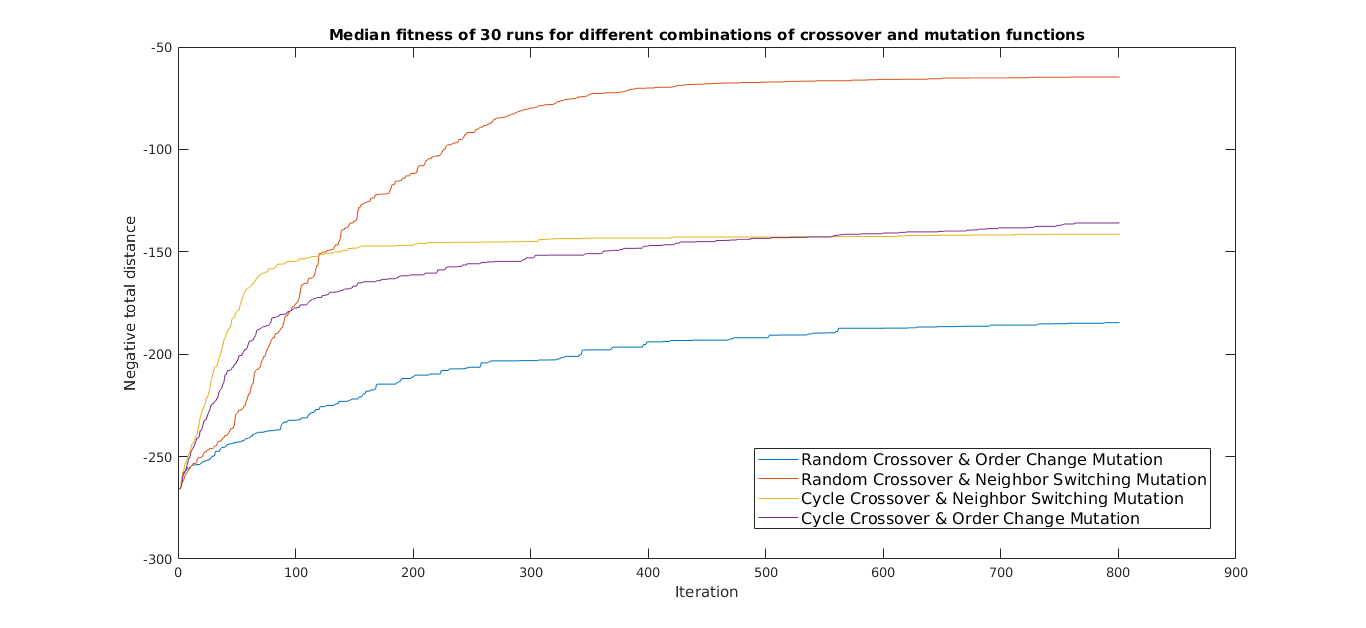
\includegraphics[width=\textwidth]{tsp_fitness_all_combinations_800.png}
\caption{\small{Evolution of median fitness in each generation over 30 runs. We tried different combinations of crossover and mutations as explained in the figure. We observe that random crossover and mutation by swapping neighbors gives us the best evolution in the fitness. The algorithm looks for maxima on the fitness landscape, thus our distance values have negative sign.}}
\label{statistics}
\end{center}
\end{figure}


%%%%%%%%%%%%%%%%%%%%%%%%%%%%%%%%%%%%%%%%%%%%%%%%%%%%%%%%%%%%%%%%%%%%%%%%%%%
\end{document}